\section{Clustering}
\smallskip \hrule height 2pt \smallskip

\begin{itemize}
	\item Unsupervised learning: detect patterns in unlabeled data. 
		Sometimes labels are too expensive, unclear, etc. to get them.
		Examples:
		\begin{itemize}
			\item group e-mails or search results
			\item find categories of customers
			\item detect anomalous program execuations
		\end{itemize}
	\item Useful when you don't know what you are looking for. 
	\item Requires a definition of "similar".  One option: small (squared) euclidean distance. 
	\item You can label then use the clusters, or use the clusters for the next level of analysis.
\end{itemize}

\subsection{K-Means}
\begin{itemize}
	\item An iterative clustering algorithm.  \hfill \\
	\item No step size.  Discrete optimization. 
	\item Hard assignments.  Each point gets classified by one and only one cluster. 
	\item will converge, but may converge on local (not global) optimum.
		\begin{itemize}
			\item Every time you start the algorithm, you could end up n a different place.
			\item Can run it a bunch of times. % week 9 audio
			\item you are running a non-convex optimization: your final output is dependent on your initialization.
		\end{itemize}
	\item you have to chose a number of clusters. 
	\item Objective: minimize the distances between each point and closest center. 
	\item You want your output to have a large distance between clusters and a small distance between points in a cluster.  (intra vs inter cluster distance).
	You want it to latch onto clumps of the data that are far apart from each other. % week 9 audio
		\begin{itemize}
			\item intra: \hfill \\
				E.g. measure $|x_i - c_i|_2^2$ for each cluster. 
			\item inter:  \hfill \\
				Dist between closest two points in different clusters. \hfill \\
				Distance between means.  \hfill \\
				Standard deviation of cluster distances. \hfill \\
		\end{itemize}
\end{itemize}	
	
Pick K random points as cluster means: $c^1, \dots, c^k$.  \hfill \\
Alternate:
\begin{itemize}
	\item Assign each example $x^i$ to the mean $c^i$ that is closest to it
	\item Set each mean $c^i$ to the average of its assigned points. 
\end{itemize}
Stop when no points' assignments change. \hfill \\

Minimizing a loss that is a function of the points, assignments, and means:
$$ L( \{ x*i \},  \{ a*j \},   \{ c*k \}) = \sum_i dist(x^i, c^{a^i})$$
Coordinate gradient descent on L.  \hfill \\

More formally: 
\begin{itemize}
	\item Data: $\{ x^j | j = 1 \dots n \}$
	\item For $ t = 1 \dots T$:  (or stop if assignments don't change): \hfill \\
		Fix means ($c$) while you change the assignments ($a$): \hfill \\
		\begin{itemize}
			\item for $ j = 1 \dots n$: (recompute cluster assignments):
				$$ a^j = \argmin_i dist(x^j, c^i)  $$ 
		\end{itemize}
	\item fix assignments ($a$) while you change the means ($c$): \hfill \\
		for $j = 1 \dots k$: (recompute cluster centers)
		$$ c^j = \frac{1}{|\{ i | a^i = j \}|}  \sum_{\{ i | a^i = j \}} x^i$$
\end{itemize}
Note:  the point y with minimum squared Euclidean distance to a set of points {x} is their mean

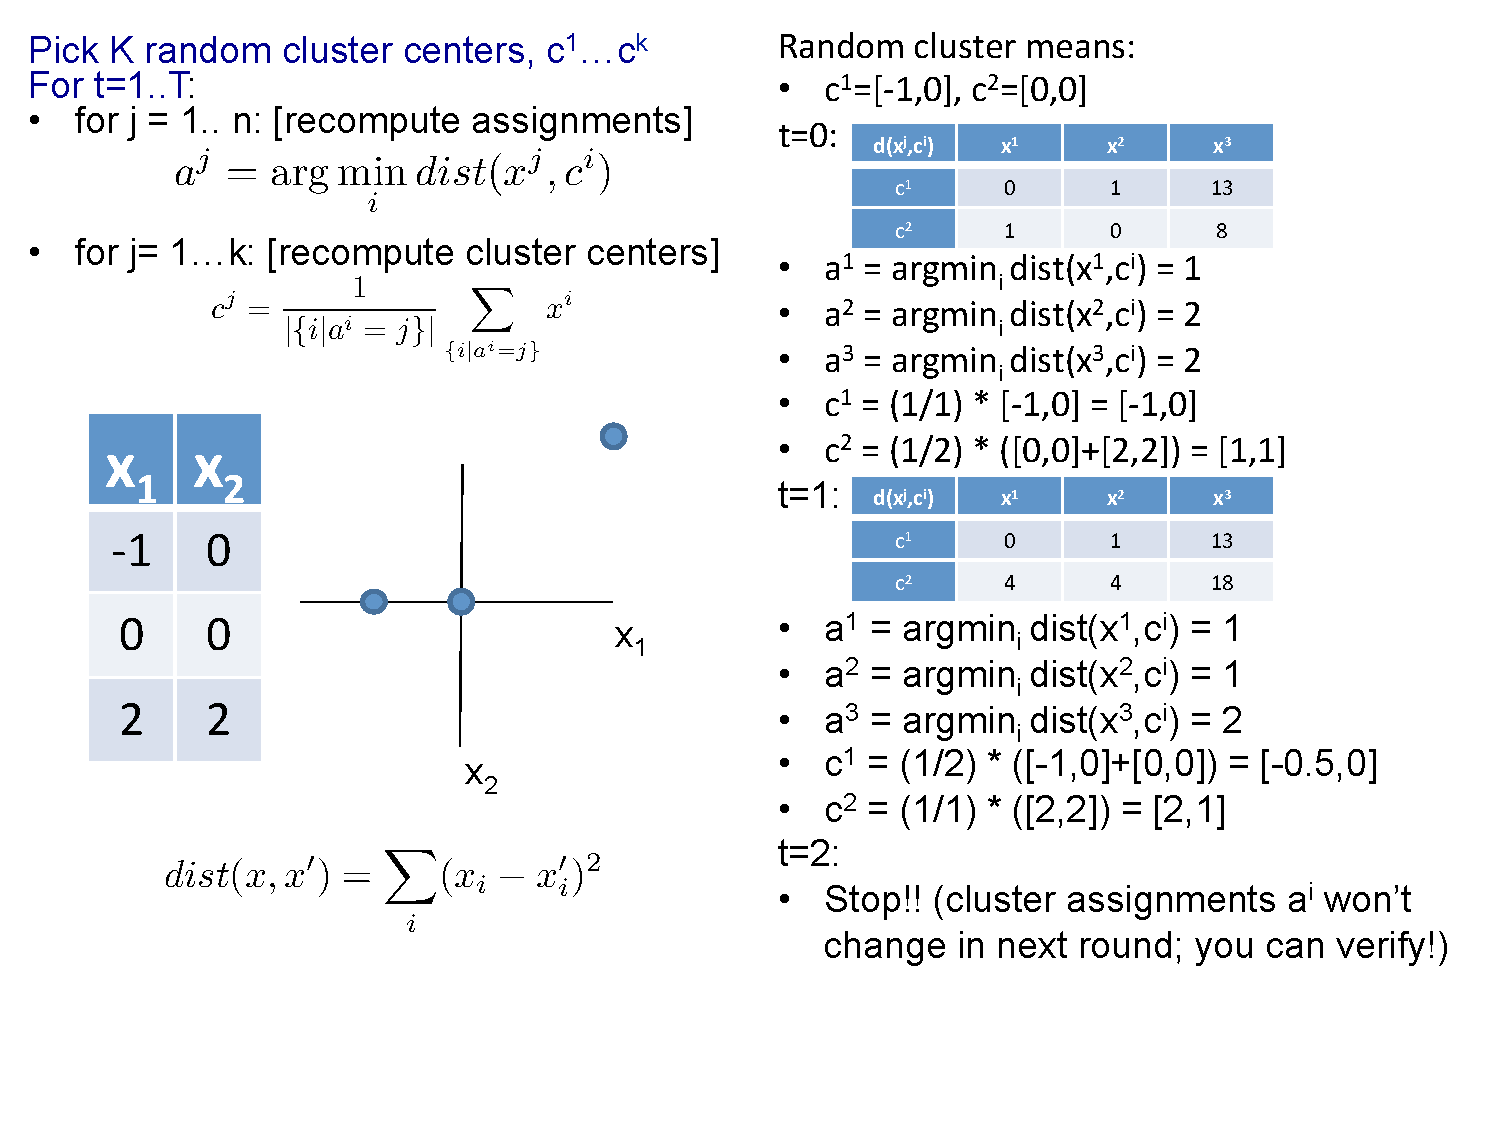
\includegraphics[width=3.6in]{figures/kmeans_algorithm_example.pdf}

\subsubsection{K-Means gets stuck in local optima.}

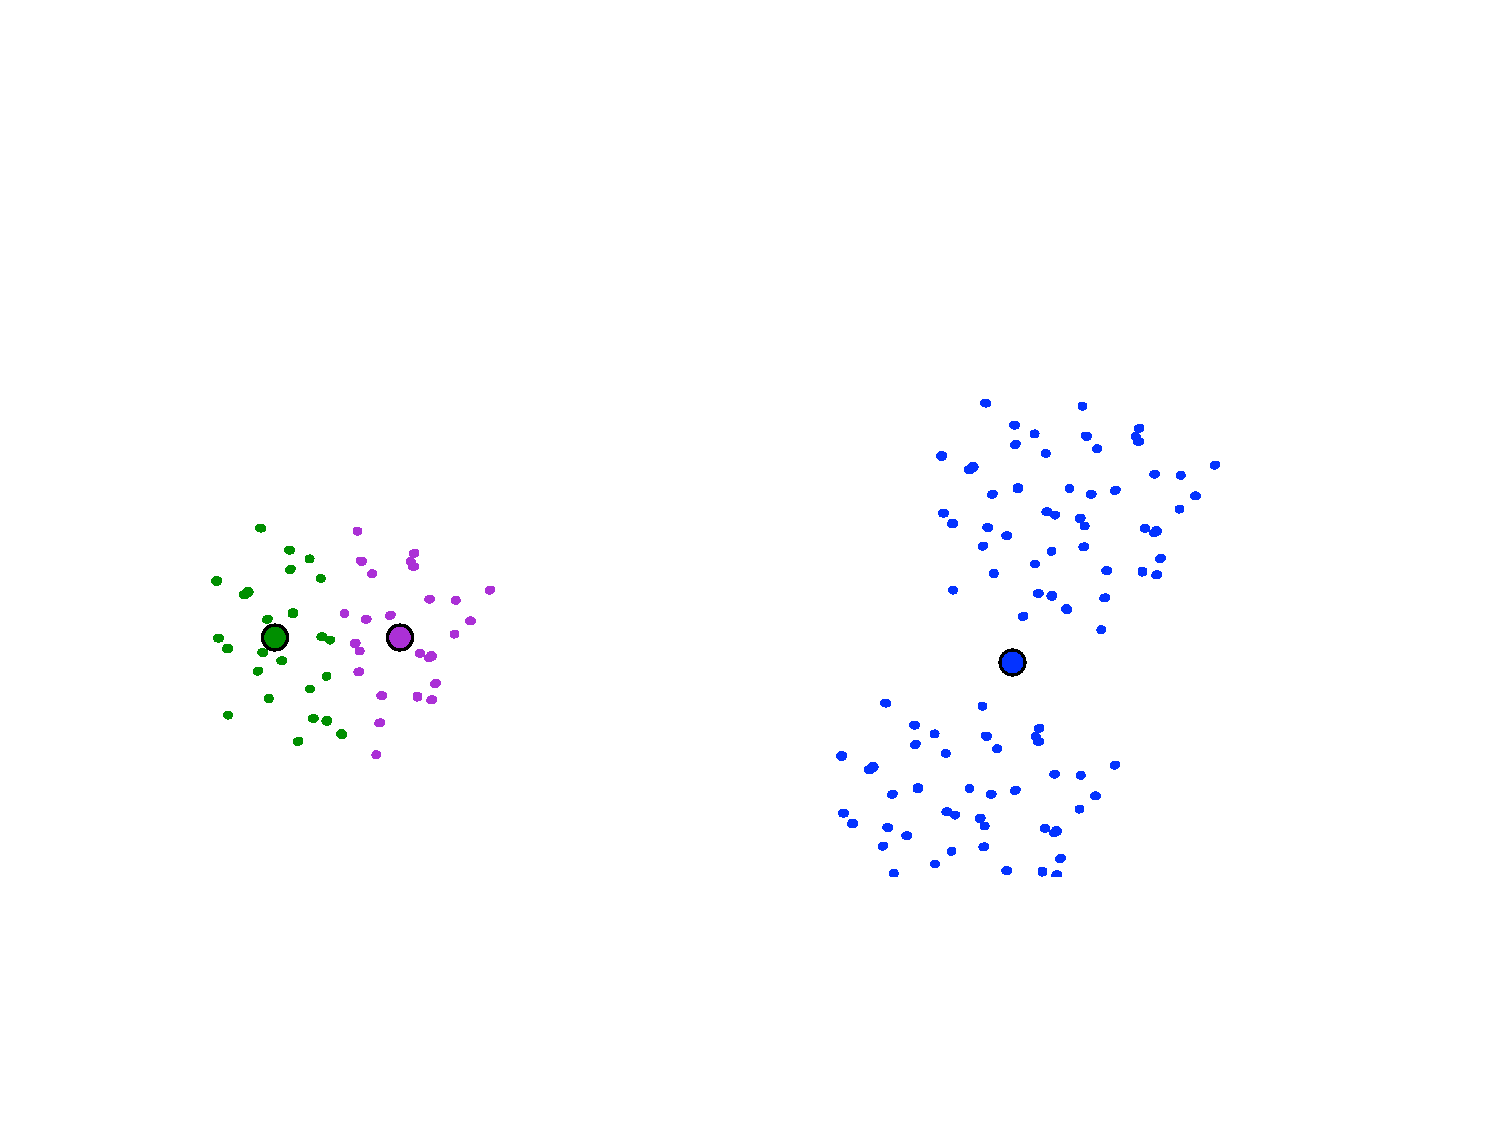
\includegraphics[width=1.8in]{figures/k-means_gets_stuck.pdf}

\subsection{Agglomerative Clustering}
First merge very similar instances. \hfill \\
Then incrementally build larger clusters out of smaller clusters. \hfill \
Limiting the number of pairs of pairs, we can control the number of clusters.
\begin{itemize} 
	\item Distance = 0 means each point is its own cluster
        \item Distances = infinity --> all in one cluster. 
\end{itemize}

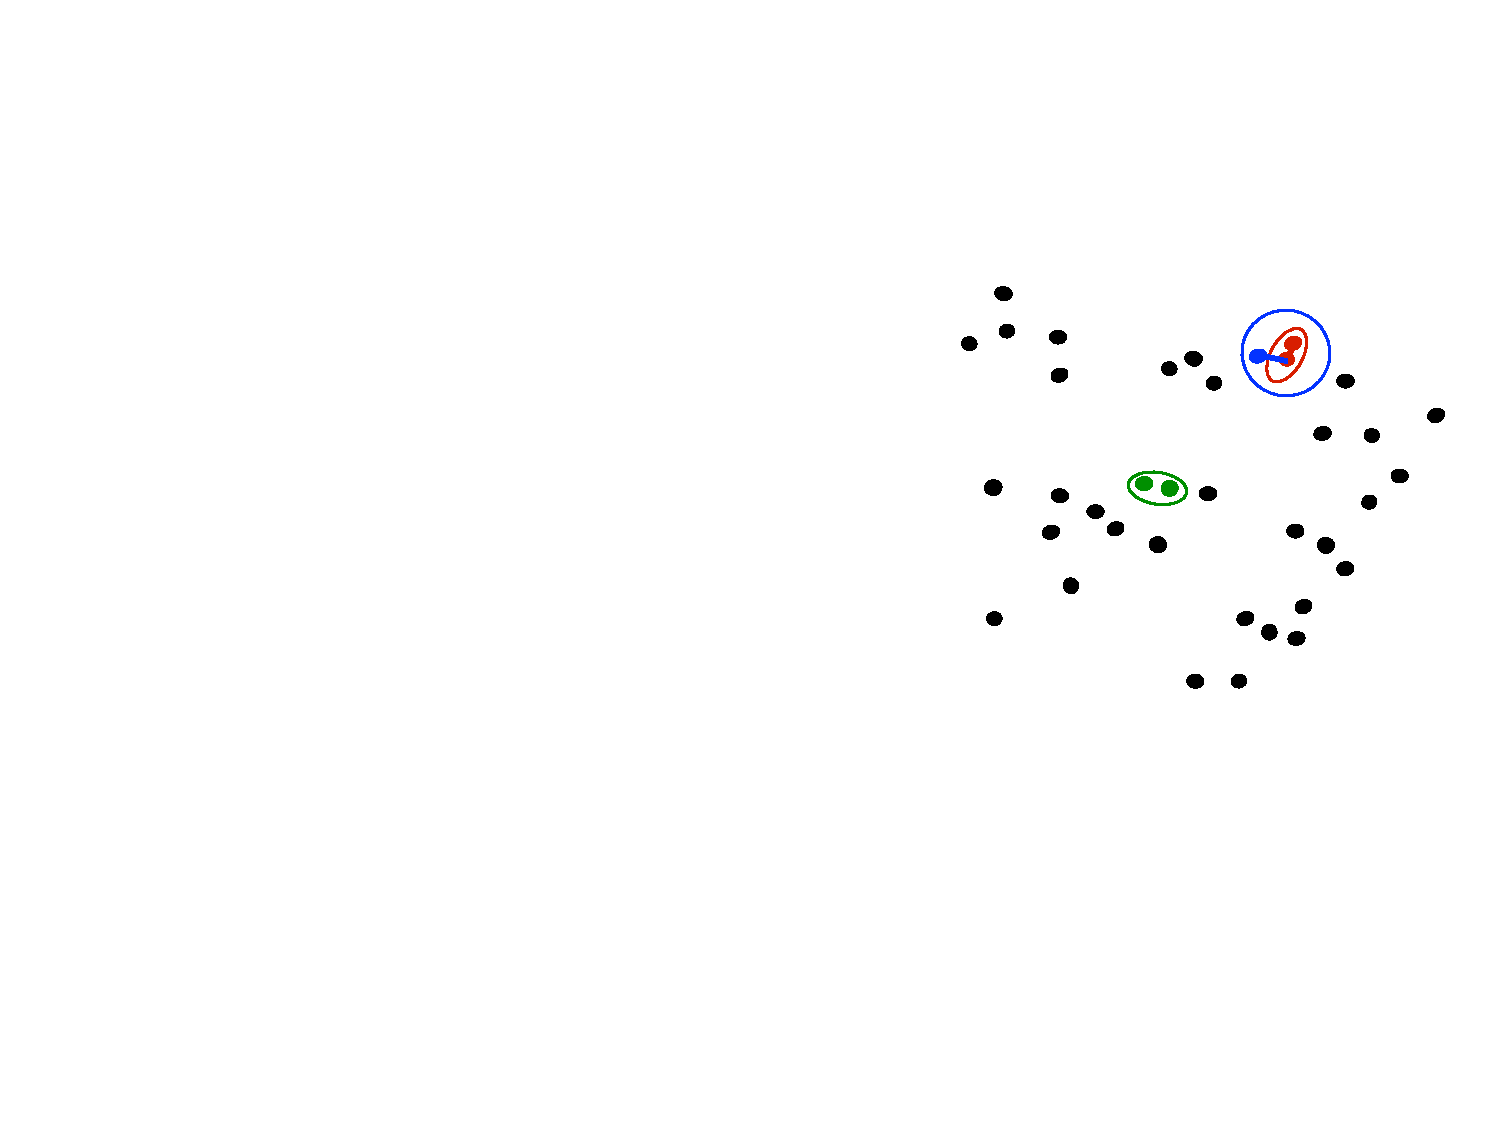
\includegraphics[width=1.0in]{figures/agg_clustering.pdf}

Algorithm:
\begin{itemize}
	\item Maintain a set of clusters.
	\item Initially each instance is its own cluster
	\item Repeat:
		\begin{itemize}
			\item pick the two closest clusters
			\item merge them into a new cluster
			\item stop when there is only one cluster left. 
		\end{itemize}
	\item produces not one clustering, but a family of clusterings represented by a dendogram.
		
		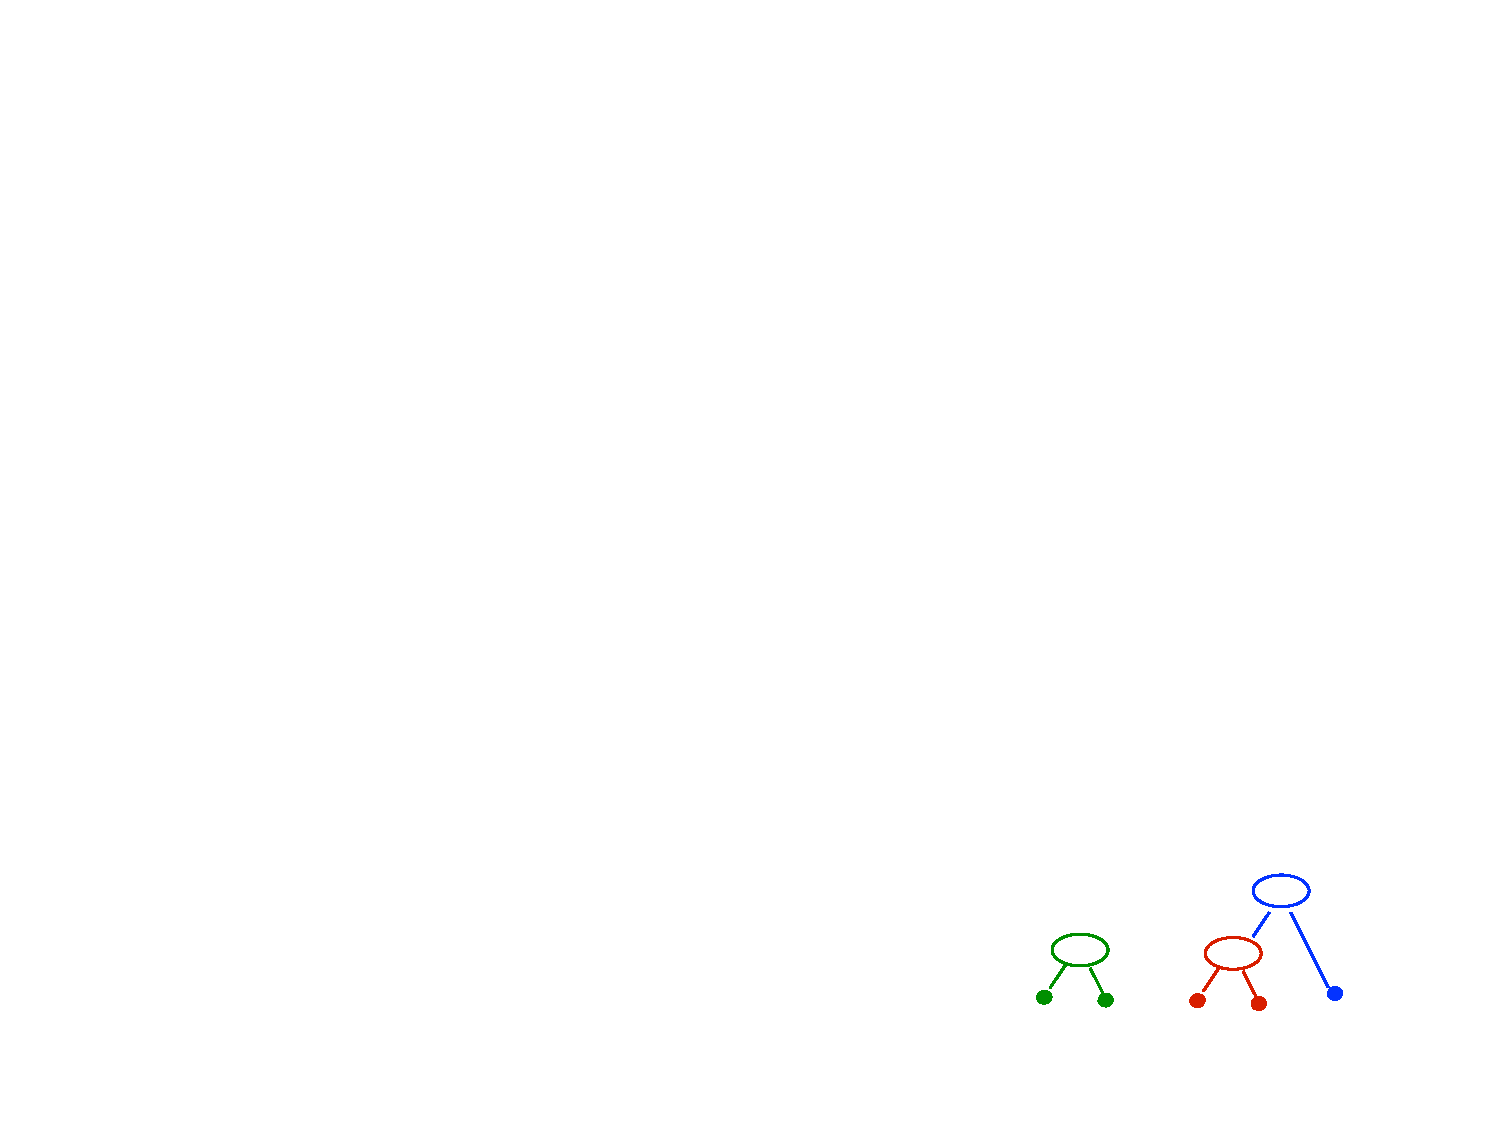
\includegraphics[width=1.0in]{figures/dendogram.pdf}
\end{itemize}

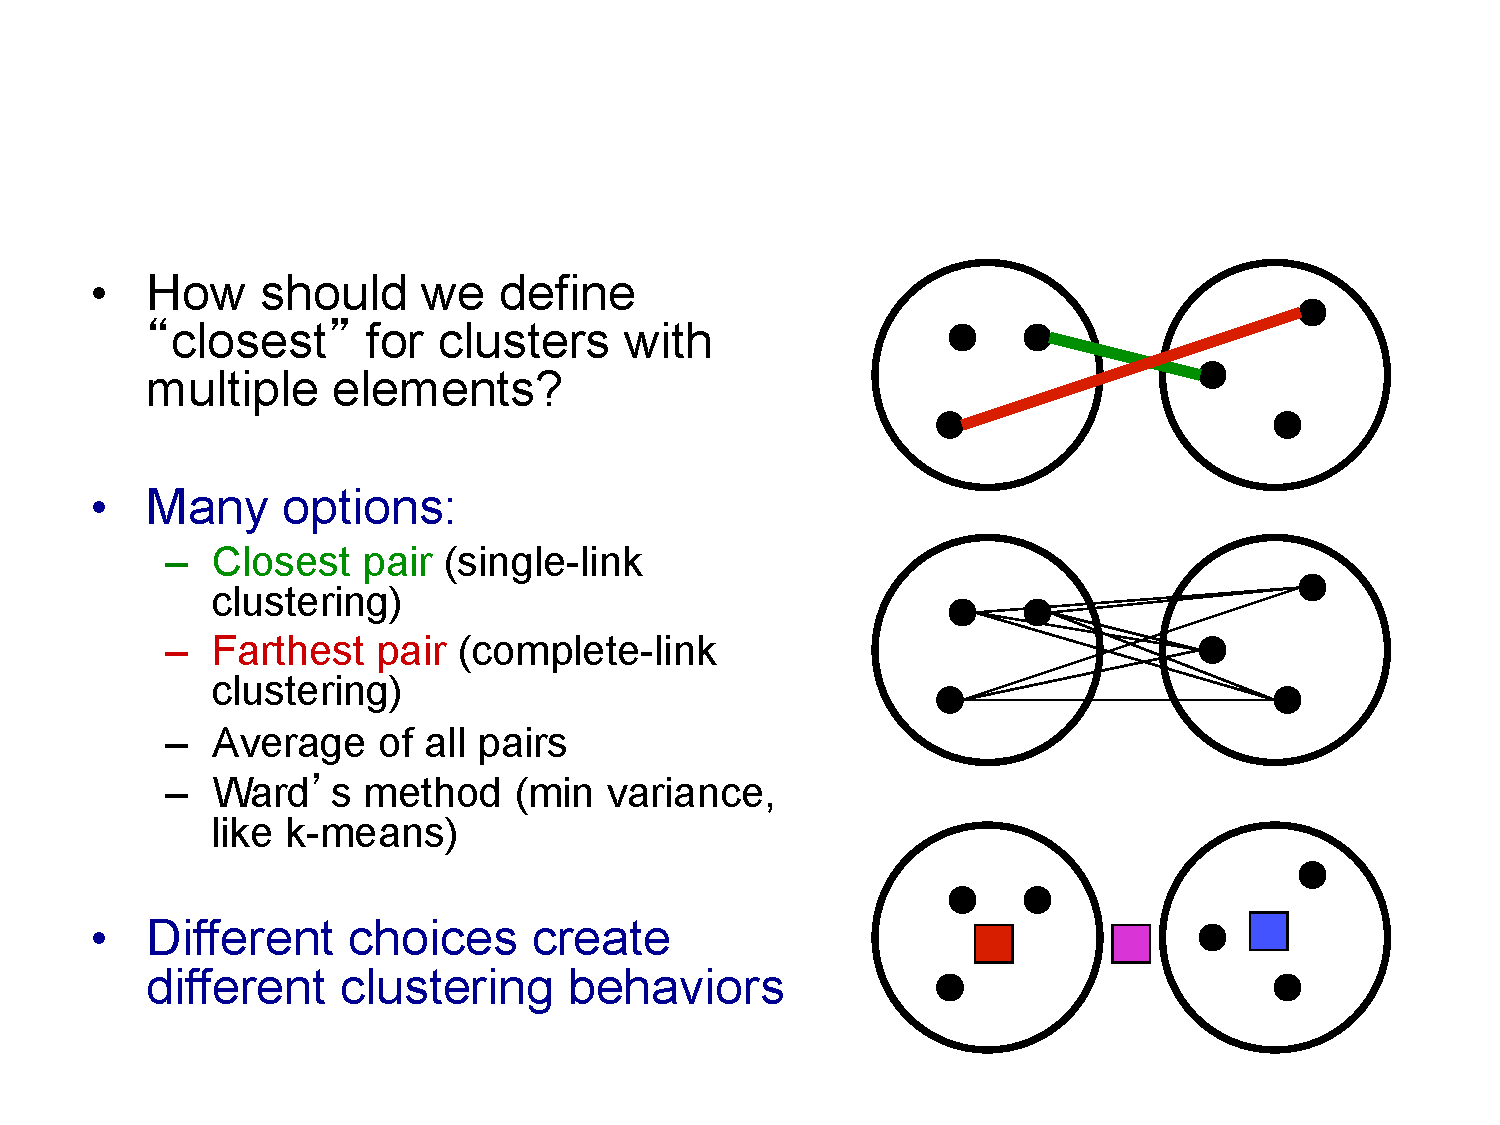
\includegraphics[width=2.7in]{figures/agglomerative_clustering_distance_options.pdf}

The intra-cluster distance: a metric of how well the clustering algorithm works
$$ S_1 = \sum_{j=1}^3 \sum_i |x_i - x_c|_2^2 + \sum_{i,j} |c_j, c_i|_2^2 $$ % wk 9 audio

You have to be extremely lucky to find a data set where the result isn't dependent on the start.

Can run it a bunch of times. % week 9 audio
For each pair of points, we have a vote:  \hfill \\
Do they belong to the same cluster? \hfill \\
Look at score from score of clustering algorithm \hfill \\
We get a full graph where edge scores are "do they belong to the same 					cluster"  (and more audio I missed?) \hfill \\
Then you need to find out which components are connected.  \hfill \\

For each pair of points, we have an edge distance.  \hfill \\
Within-cluster edges should be strong edges.    \hfill \\
This strength should be common across clustering results.  \hfill \\
Cut the graph into three pieces.    \hfill \\
The score of the cut is the summation of the edges you break.   \hfill \\
Cutting edges with small scores is good.   \hfill \\


\subsection{Probabilistic Clustering}
\begin{itemize}
	\item Can use a probabilistic model that allows cluster overlaps, clusters of different sizes, etc.
	\item You can tell a generative story for the data.  \hfill \\
		$P(X|Y) P(Y)$ is common. 
	\item The challenge: estimate model parameters without labeled data. 
\end{itemize}

\subsection{Gaussian Mixture Models}
\begin{itemize}
	\item We have clumps of data. Each clump is described with a gaussian.  % wk 10 audio
	\item Like softening k-means.  You belong to cluster 1 with a score of 0.1, cluster 2 with score of 0.3, cluster 3 with score of 0.6
	\item Think of clusters as probabilistic. 
	\item Assume m-dimensional data points.
	\item P(Y) is still multinomial, with k classes.
	\item $P(\mathbb{X} | Y=i), i=1 \dots k$ are $k$ multivariate Gaussians.
		\begin{itemize}
			\item mean $\mu_i$ is a m-dimensional vector.
			\item variance $\Sigma_i$ is an $m$ by $m$ matrix.
			\item $|x|$ is the determinant of matrix x. 
		\end{itemize}
\end{itemize}

$$ P(X=x | Y=i) = \frac{1}{\sqrt{(2 \pi)^m | \Sigma_i |}} \exp \left(  \frac{1}{2}(x - \mu_i)^T \Sigma_i^{-1} (x- \mu_i) \right) $$

\subsubsection{GMM is not Gaussian Naive Bayes}
(We did GNB before logistic regression) \hfill \\
Gaussian Naive Bayes : multinomial over clusters $Y$, Gaussian over each $X_i$ given $Y$:
$$ P(Y_i = y_k) = \theta_k $$
(Again, $\theta$ is the model parameters)
$$ P(X_i = x | Y = y_k) = \frac{1}{\sigma_{ik} \sqrt{2 \pi}} \exp \left(  \frac{-(x - \mu_{ik}^2}{2 \sigma_{ik}^2} \right) $$
? Would assume the input dimensions $X_i$ do not co-vary. \hfill \\

If the input dimensions $X_i$ do co-vary, we can use Gaussian Mixture Models. 

\subsubsection{Gaussian Mixture Model Assumption}
We want to do something like MLE but now we have multiple Gaussians. \hfill \\
You don't know which label should be used for each data point(which is red, blue, green). \hfill \\
Need to guess $k$ Gaussians without knowing the $\mu$s.  \hfill \\

You can marginalize: \hfill \\
Model probability without knowing who belongs to who: marginalize over all possible y values.   \hfill \\
You are estimating $P(X|Y)$, but you don't know $Y$.   \hfill \\
You can get rid of $Y$ and get $P(X)$ by summing over $y_i$.  \hfill \\
Get $Y$ out of the equation by summing over all possible values. \hfill \\
If it was a probability table, we would be losing a column. \hfill \\


\begin{itemize}
	\item $P(Y)$: there are $k$ components
	\item $P(X | Y)$: each component generates data from a Gaussian with mean $\mu_i$ and covariance matrix $\Sigma_i$
	\item Assume each of the features are independent of each other. \hfill \\ % week 10 audio
		Then can write down $P(X|Y)$ as prod of $P(X_i | Y)$.  \hfill \\ % week 10 audio
        		Each of them will be a Gaussian distribution. \hfill \\  % week 10 audio
	\item  Can encode the whole $P(X|Y)$ with a multi-dimensional gaussian. \hfill \\  % week 10 audio
		For 2D data, this gives a circle.  \hfill \\  % week 10 audio
		For 3D data, this gives a bump.  \hfill \\  % week 10 audio
		 When we go to 100-dim space, we also have a mu.   \hfill \\  % week 10 audio
		 	Distribution is 100-dimensional. \hfill \\  % week 10 audio
			Sigma in 100-dim space is 100 by 100 covariance matrix. \hfill \\  % week 10 audio
\end{itemize}

Each data point is sampled from a \textbf{generative process}
\begin{itemize}
	\item Pick a component at random: \hfill \\
		choose component $i$ with probability $P(y=i)$
	\item Datapoint $\sim N(\mu_i, \Sigma_i)$
\end{itemize}

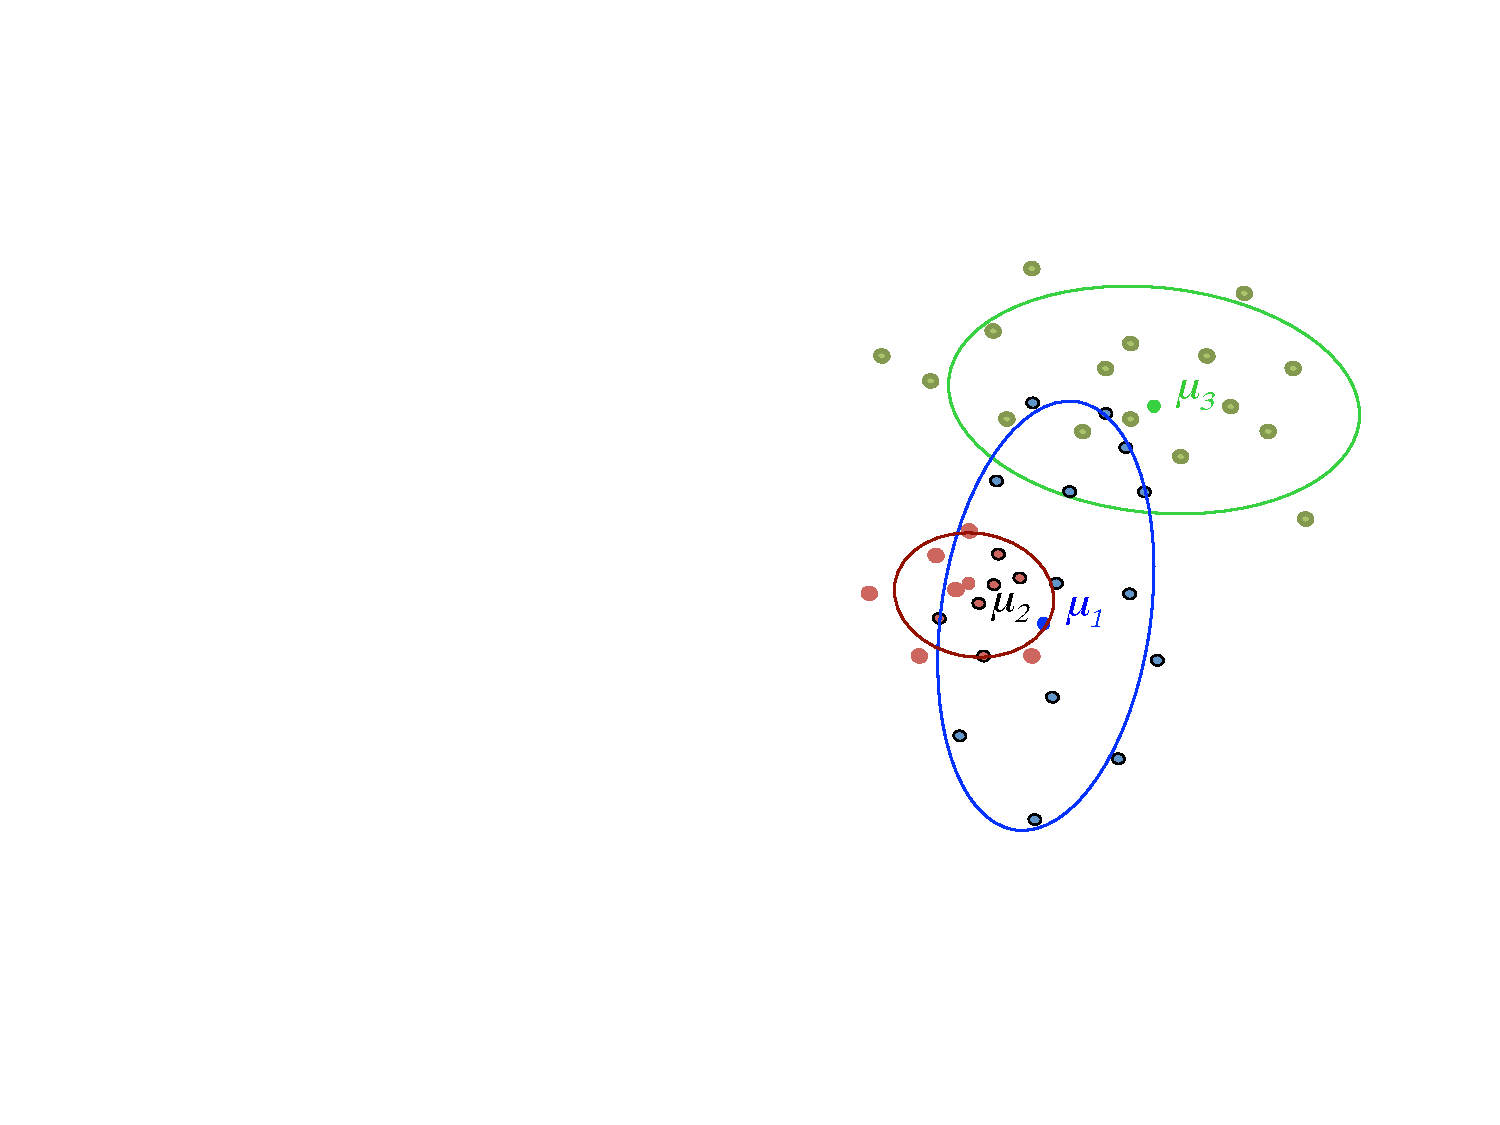
\includegraphics[width=1.0in]{figures/GMM_cartoon.pdf}

\subsubsection{Supervised MLE for GMM}
(Detour/review) \hfill \\

How do we estimate parameters for Gaussian Mixtures with fully supervised data? \hfill \\
Define objective and solve optimization: \hfill \\
From above: 
$$ P(X=x | Y=i) = \frac{1}{\sqrt{(2 \pi)^m | \Sigma_i |}} \exp \left(  \frac{1}{2}(x - \mu_i)^T \Sigma_i^{-1} (x- \mu_i) \right) $$
And we know $ \displaystyle \mu_{ML} = \frac{1}{n} \sum_{i=1}^n x^i$ and $ \displaystyle \Sigma_{ML} = \frac{1}{n} \sum_{i=1}^n (x^i - \mu_{ML}) (x^i - \mu_{ML})^T$ \hfill \\

But we don't know Y, so we can't do that.  \hfill \\

Instead, we maximize the marginal likelihood.  (marginal means a variable is integrated out).
$$ \argmax_{\theta} \prod_i P(x^j; \theta) = \argmax \prod_j \sum_{i=1}^k P(y^j=i, x^j; \theta) $$

This is always a hard problem.  \hfill \\
There is usually no closed form solution.  \hfill \\
Even when $P(X, Y; \theta)$ is convex, $P(X; \theta)$ generally isn't.  \hfill \\
For all but the simplest  $P(X; \theta)$, we will also have to do gradient ascent, in a big messy space with lots of local optima.   \hfill \\

\subsubsection{Simple GMM example: learn means only}
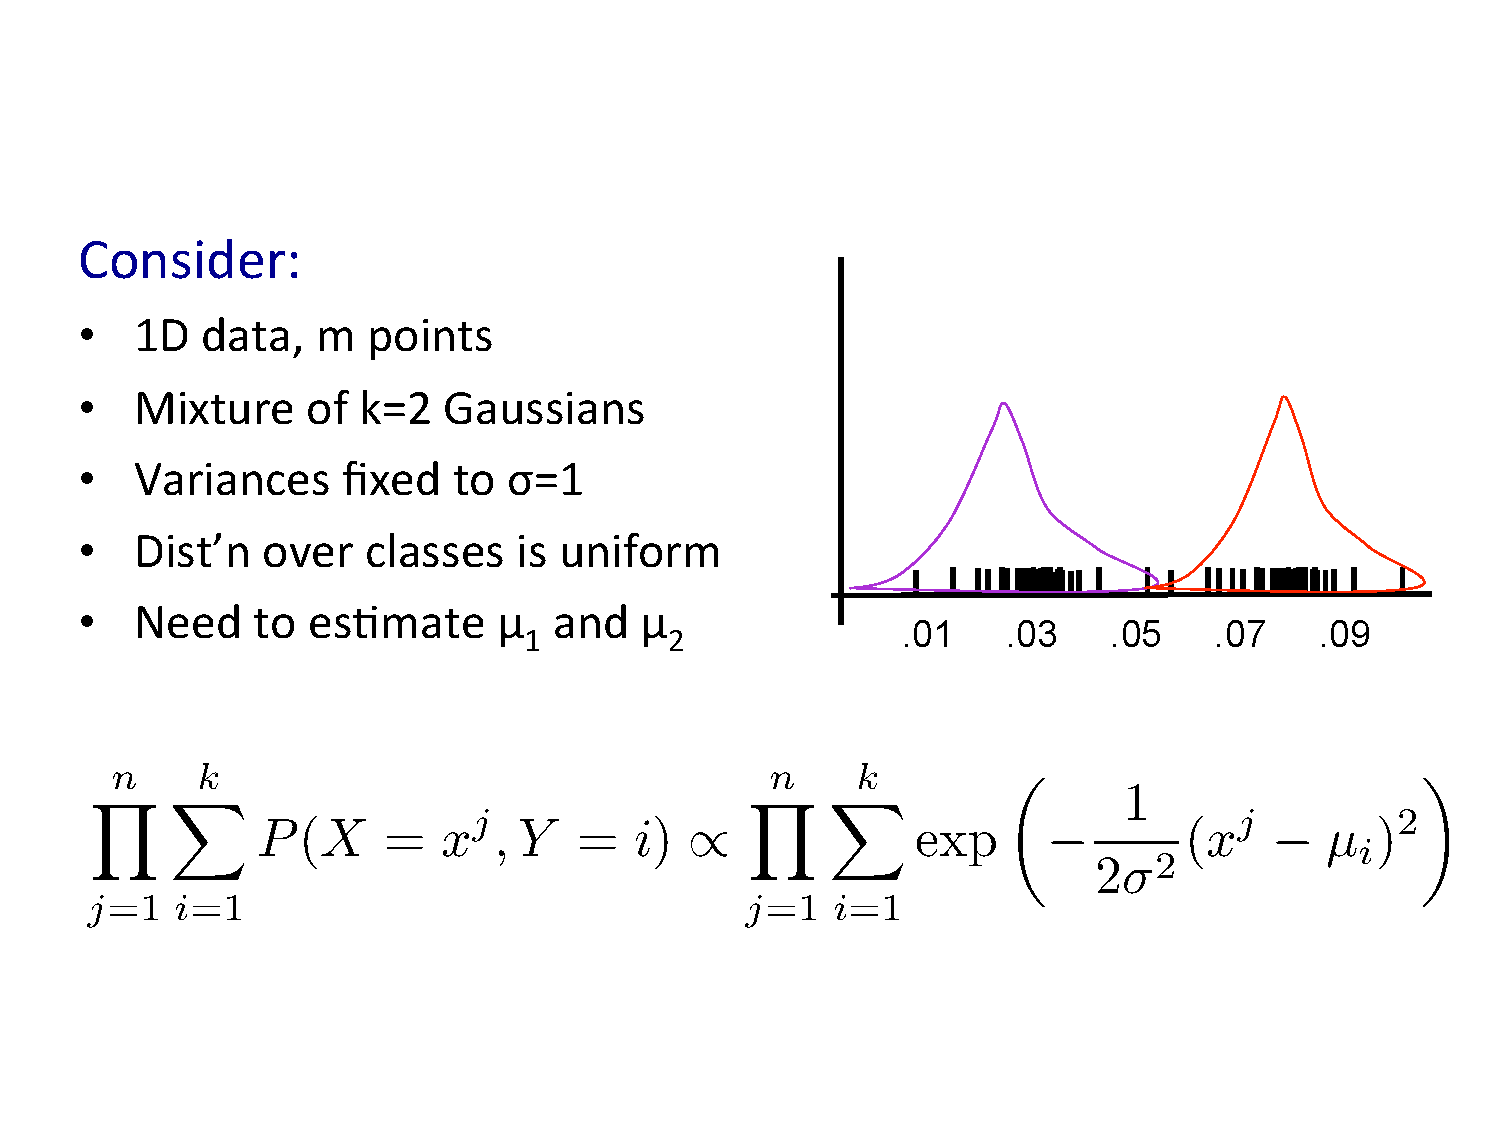
\includegraphics[width=2.5in]{figures/gmm_for_means_only.pdf}

We solve this using EM below. 

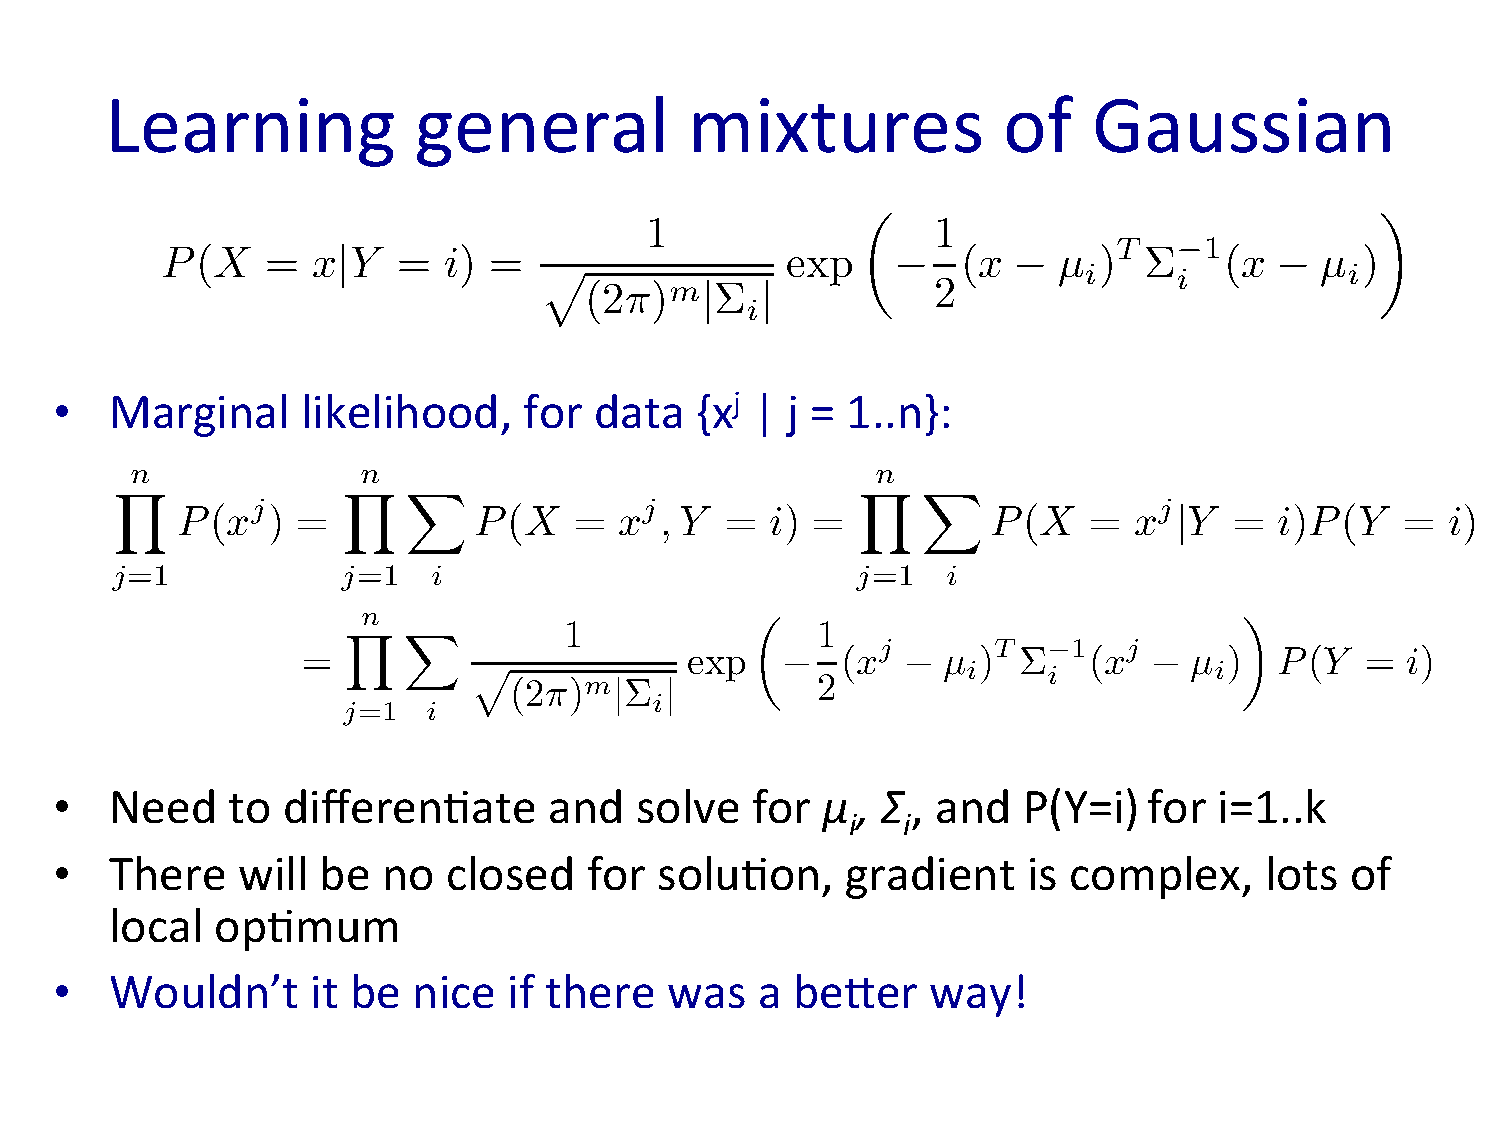
\includegraphics[width=2.5in]{figures/learning_general_mixtures_of_Gaussians.pdf}

